\documentclass{report}

\usepackage[italian]{babel}
\usepackage[utf8]{inputenc}
\usepackage[hidelinks]{hyperref}
\usepackage{graphicx}
\usepackage[font=small,labelfont=bf]{caption}
\usepackage{setspace}
\onehalfspacing

\graphicspath{ {../assets/} }

\title{Report sul protocollo GREEN-WUP}
\author{Leonardo Emili}

\begin{document}
\maketitle
\tableofcontents

\chapter{GREEN-WUP}
\section{Il protocollo GREEN-WUP}

Il protocollo GREEN-WUP si inserisce nel contesto dei protocolli delle cosiddette \emph{green wireless sensor network} e pone tra i suoi principali
obiettivi l'efficienza energetica dell'intera rete. Esso impiega le tecnologie di wake up radio, energy harvesting e semantic addressing. Inoltre, è
di tipo \emph{converge casting} ed è basato sull'assegnazione di hop count a ciascun nodo per poter distribuire i pacchetti dati
all'interno della rete.\\

Esso si articola in due fasi principali: in primo luogo avviene la fase di \emph{interest dissemination} dove si definisce la
topologia della rete da rispettare affinchè i nodi realizzino un corretto flusso di scambio dati; successivamente si assume che gli indirizzi di
wake up siano stati assegnati e si procede con lo scambio di dati che è governato da sequenze di wake up che vengono utilizzate per
risvegliare i nodi della rete.\\

Inizialmente il sink node invia un primo \emph{command packet} che viene successivamente distribuito ai nodi sensori utilizzando l'algoritmo di \emph{flooding}.
L'obiettivo di questo processo è di assegnare a ciascun nodo della rete un valore di hop count secondo un algoritmo iterativo: questo
avrà valore 0 nel solo caso del sink node, altrimenti assume un valore $h$ se $h-1$ è il valore di hop count del nodo precedente. Al termine
di questa fase ciascun nodo sarà fornito di un indirizzo di wake up $w=w_{h}w_{e}$ della lunghezza di 8 bit, con $w_{h}$ definito dal valore di hop
count $h$ e $w_{e}$ che rappresenta la classe energetica del nodo. In particolare, ciascun nodo considera
l'energia disponibile come quella rimamente nelle batterie assieme a quella derivata da sorgenti esterne. In definitiva, la codifica del suffisso $w_{e}$
viene calcolata a partire dalla discretizzazione in $k$ classi della disponibilità energetica di un nodo, dove $k$ rappresenta il numero delle classi
disponibili.\\

Ciascun nodo è in grado di calcolare i propri indirizzi di wake up. Nel caso di GREEN-WUP sono presenti due indirizzi: un primo indirizzo che identifica
univocamente il nodo nella rete e rimane invariato nel tempo, e un secondo che tiene conto del valore di hop count e che sarà periodicamente aggiornato
in base alla disponibilità energetica corrente. Questa idea realizza il principio del semantic addressing poiché in questo scenario
è possibile far riferimento ad un sottoinsieme di nodi della rete a partire dai loro valori di hop count e da quello della classe energetica. \\

%image source: https://www.researchgate.net/figure/Topology-of-wireless-sensor-network-and-hop-count-of-sensors_fig7_285956270
\begin{figure}
    \begin{center}
        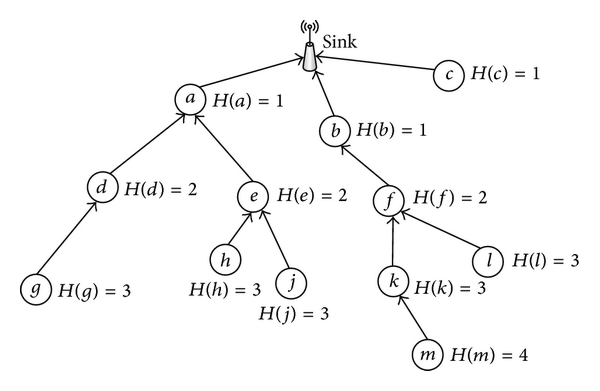
\includegraphics[scale=1.7]{hop-count-algorithm.png}
        \caption{Topologia della rete a seguito dell'assegnazione degli hop count.}
    \end{center}
\end{figure}

In definitiva, se un nodo deve inviare un pacchetto dati può farlo seguendo degli step fondamentali: una prima fase di comunicazione con i nodi elegibili
alla ritrasmissione del pacchetto; una seconda fase di selezione del nodo che si farà carico della richiesta; infine la fase di trasmissione del pacchetto,
a seguito della quale verrà inviata una conferma a certificare l'avvenuta ricezione dello stesso.\\

In particolare,
consideriamo un nodo $a$ non a diretto collegamento col sink node, dunque si ha un valore di hop count $l>1$. Al momento della richiesta di trasmissione dati,
$a$ prepara una sequenza di wake up $w$ con semantic addressing, scegliendo inizialmente la massima classe energetica $k$, e verifica facendo
\emph{carrier sensing} che il canale di comunicazione sia libero. Se il canale è libero allora procede inviando la sequenza di wake up con semantic addressing
che sveglierà tutti e soli i nodi con classe energetica massima. Esso attende un contingente di tempo necessario affinchè i nodi destinatari, siano
questi $B_1, B_2, \ldots B_n$ possano accendere le antenne principali (RX) ed invia in broadcast un pacchetto \emph{Request To Send} (RTS), all'interno
del quale viene incluso l'indirizzo di wake up che indentifica univocamente $a$. Al momento della ricezione, i nodi $B_1, B_2, \ldots B_n$ spengono la
radio principale (SLEEP). Successivamente questi svegliano il nodo $a$, utilizzando la sequenza di wake up contenuta nel pacchetto RTS ricevuto, ed in
seguito inviano un pacchetto \emph{Clear To Send} (CTS), in cui è presente l'indirizzo di wake up che identifica univocamente gli stessi. Per evitare
collisioni durante l'invio del pacchetto CTS i nodi ne rimandano la trasmissione utilizzando un tempo di \emph{jitter} randomico.
Al momento della ricezione del primo CTS $a$ seleziona il nodo $B_i$ per la ricezione del pacchetto dati. Quindi $a$ verifica che il canale di comunicazione
sia libero ed in caso positivo sveglia $B_i$ utilizzando la sequenza di wake up contenuta nel pacchetto CTS in questione ed in seguito il \emph{DATA packet}.
Dunque, $B_i$ ricevuto il pacchetto dati invia un \emph{acknowledgement packet} (ACK) ad $a$, va a dormire e prosegue la
ritrasmissione del pacchetto ricevuto sino ad arrivare al sink node. Infine $a$ va a dormire in attesa di svolgere una nuova operazione.\\

Il design del protocollo prevede che ciascun nodo consideri dapprima i soli nodi con classe energetica più alta. Se, a seguito di un numero massimo di tentativi,
questo non riesce a mettersi in contatto con nessuno di loro allora si procede considerando la classe energetica immediamente inferiore e si ripete
l'intera procedura. Inoltre, nel caso in cui il nodo sorgente è a diretto contatto con il sink node ($l=1$), il protocollo prevede che
lo scambio dei pacchetti DATA e del relativo ACK avvenga senza avviare la procedura di scambio di RTS e CTS, in quanto superflua la
selezione di un nodo intermedio.\\

\section{Le problematiche emerse}

GREEN-WUP impiega jitter puramente randomici al momento dell'invio dei pacchetti CTS per tentare di evitare che avvengano collisioni durante
la trasmissione. In questo modo, i nodi inviano un pacchetto CTS il cui tempo di ricezione dipende unicamente dal valore di jitter
considerato e dalla distanza dei singoli dal nodo ricevente, in quanto viene considerato il tempo di trasmissione un'ulteriore ritardo nella
trasmissione pacchetto. La scelta \emph{greedy} secondo cui un nodo trasmette un pacchetto ad un certo tempo $t+jitter$ non aggiunge alcuna
informazione sullo stato dello stesso. Si tratta di una scelta per alcuni aspetti ragionevole, in quanto non aggiunge overhead alla trasmissione
del pacchetto, ma che non garantisce che il percorso scelto nella rete sia il migliore in termini di efficienza e di costo energetico. Un nodo
potrebbe essere selezionato come nodo intermedio seppur trovandosi in uno stato di scarsa disponibilità energetica. Considerando inoltre che
ciascun nodo è dotato di un buffer di ricezione con capacità limitata, è possibile che un nodo sia selezionato come nodo intermedio pur non
potendo bufferizzare nuovi pacchetti a seguito di un riempiemento della coda (\emph{buffer overflow}).\\

Inoltre, durante lo scambio di RTS e CTS viene scelto un nodo che opererà da intermediario per la ricezione del pacchetto destinato
al sink node. I nodi sono considerati sulla base della loro posizione rispetto al sink node (HOP COUNT) e alla loro disponibilità energetica corrente.
Tuttavia questa procedura non garantisce che tutti i nodi svegliati siano abilitati alla ricezione di nuovi pacchetti, poichè, in maniera simile a
quanto sopra descritto, un nodo può essere nella condizione di non poter ricevere nuovi pacchetti, verificandosi quindi sprechi di energia ed
ulteriori ritrasmissioni per far recapitare il pacchetto. In generale, l'approccio di GREEN-WUP non garantisce l'efficienza energetica della rete,
nè tantomeno permette di ottenere latenze ottimali. Si osservi come un nodo che è impegnato nel processamento di un pacchetto possa essere selezionato
come nodo intermediario rispetto ad un altro che si trova alla stessa distanza dal sink node (stesso hop count) e che ha coda di ricezione vuota, se questo
ha, ad esempio, classe energetica immediamente inferiore al nodo in questione. \\

Osservando in dettaglio il comportamento dei nodi durante la fase di selezione del nodo intermediario si può notare un dettaglio degno di nota.
Al momento della ricezione di una sequenza di wake up con semantic addressing da parte di un nodo, questo attiverà la radio principale e si metterà in
ascolto di nuovi dati. Questo accade poichè la risposta al trigger della sequenza di wake up genera un evento in ciascun nodo che lo porta inevitabilmente
ad attivare la radio principale. Se tuttavia i nodi candidati a svegliarsi in seguito alla ricezione del messaggio di wake up sono numerosi, si può avere uno
spreco energetico considerevole. Un'analisi del comportamento di GREEN-WUP ci permette di osservare come i nodi riceventi non hanno possibilità di scegliere l'azione
intrapresa in seguito alla ricezione di un messaggio di wake up. Essi semplicemente reagiscono al messaggio ricevuto e si preparano alla ricezione di un
eventuale pacchetto dati. Analogamente alla prima problematica emersa, la scelta da parte di un nodo di svegliarsi è effettuata senza considerare lo stato dello
stesso e può portare a consumi energetici superflui.

\section{Soluzioni proposte e risultati}

Le proposte avanzate sono state testate mediante una versione particolare del framework \emph{GreenCastalia} che supporta \emph{wake up radios}
e \emph{energy harvesting}. I risultati e i dati di seguito forniti sono considerati su un numero minimo di simulazioni 
necessario a fornire veridicità alle considerazioni affermate.\\

In questo lavoro si propone una variante del protocollo di base di GREEN-WUP che adotta alcune modifiche in risposta alle problematiche emerse nel capitolo
precedente. Nel seguito, per ciascuna problematica si descrivono le modifiche adottate, le implicazioni e i risultati che questi cambiamenti hanno comportato.\\

La variante proposta risolve il precedente problema della mancanza di stato nella formulazione del valore di jitter considerando lo stato energetico
corrente del nodo e lo stato della sua coda di ricezione. In particolare, un nodo sarà tanto più prono a ricevere e reinstradare un pacchetto quanto
più è alta è la sua disponibilità energetica e di ricezione di nuovi pacchetti. Un nodo $j$ risponde ad un pacchetto RTS inviando un pacchetto CTS
ad un tempo $t+\delta$, con $\delta$ così definito:

$$ \delta= (1-e_{j}) \cdot k \cdot \delta_{M} + b_{j} \cdot l \cdot \delta_{M} + \delta_{r} \quad ,$$

con $e_{j}$ la frazione di energia residua del nodo corrente, $b_{j}$ lo stato di occupazione del buffer, $\delta_{M}$ il massimo delay consentito,
$\delta_{r} < \delta_{M}$ un valore randomico ed infine $k \geq 0$ e $l \geq 0$, con $k+l=1$, che regolano il contributo di ciascun elemento.\\

La presenza di un offset randomico non influisce sulla correttezza dell'approccio impiegato. Senza perdita di generalità possiamo considerarlo come una
costante dal momento che il suo unico scopo è quello di introdurre un evento aleatorio al fine di evitare le collisioni derivate dall'invio di pacchetti CTS
nello stesso momento da parte di nodi nello stesso stato (pari energia residua e stato del buffer). Così facendo il jitter scelto aumenta al crescere
delle due componenti considerate. Si noti come nell'implementazione si è scelto di dare pari peso ad entrambe le componenti ($k=1/2=l$) per favorire il
tradeoff di bassi valori per la latenza e contemporaneamente diminuire i consumi energetici della rete.\\

Un altro obiettivo della variante del protocollo di base è quello di limitare i consumi energetici della rete dovuti a risvegli non necessari dei nodi
della rete. Quindi, l'idea del semantic addressing sulla quale si basa il protocollo GREEN-WUP viene espansa introducendo lo stato del buffer di ricezione dei nodi
destinatari. L'indirizzo di wake up che viene inviato per svegliare i nodi prima consisteva nei soli valori di hop count e della classe energetica target, mentre ora
viene modificato nel formato: $1BBHHHEE$. Con $B$ che rappresenta la classe dello stato del buffer di ricezione del nodo, $H$ che denota l'hop count ed
$E$ che rappresenta la classe energetica.
L'aggiunta dei bit che codificano lo stato del buffer permettono di selezionare dapprima i nodi con classe energetica superiore che siano contemporaneamente disponibili
alla ricezione di nuovi pacchetti. Da questa modifica derivano due principali benefici: il fenomeno di buffer overflow sopra descritto viene mitigato in quanto il nodo
che ha diversi pacchetti bufferizzati sarà considerato solo dopo i nodi che hanno meno pacchetti nel loro buffer di ricezione. Inoltre, migliora
le performance della rete dal momento che i nodi saranno considerati in ordine a partire da quelli con più alta disponibilità ad accogliere nuovi pacchetti sino
a quelli che attualmente ne hanno bufferizzati diversi.\\

Nella versione base del protocollo ciascun nodo risponde alla ricezione di un messaggio di wake up a lui destinato attivando la radio principale e mettendosi
in attesa di ricevere nuovi pacchetti. Nella versione qui proposta si introduce la possibilità da parte del nodo di prendere la decisione se svegliarsi o meno.
In particolare, si utilizzano \emph{energy predictor} per studiare le predizioni dell'energia derivata da sorgenti esterne al fine di determinare se un nodo sarà o
meno nelle condizioni di potersi svegliare. La decisione viene presa dal nodo in questione in maniera del tutto indipendente dal resto della rete e basa interamente
la sua scelta in base a quanta energia sarà in grado di derivare da sorgenti esterne quali pannelli solari o turbine eoliche. Nel dettaglio, al momento
della ricezione della sequenza di wake up il nodo sceglie con una probabilità $p$, che è direttamente proporzionale al valore di energia predetto,
se questo dovrà attivare la radio principale oppure rimanere inattivo (SLEEP). L'idea in questo caso è che una sequenza di wake up può interessare più nodi
in ricezione, e dal momento che al termine della procedura solamente un nodo sarà selezionato come intermediario allora questa decisione può essere influenzata dalla
disponibilità energetica dei nodi stessi in un certo istante \emph{T}. Si noti come nel caso migliore la modifica apportata comporti che un numero minore di nodi
rispetto alla versione originale sia coinvolto durante la fase di scelta del nodo intermedio, con conseguente diminuizione dei costi energetici e latenze dovute a
possibili ritrasmissioni. Può tuttavia accadere che il nodo candidato alla ricezione non si svegli mai in quanto il valore randomico $r$ non supera mai la
soglia $t$ da noi fissata. Ma questo accade con una probabilità che dipende dal numero di possibili ritrasmissioni $n$ per livello e che diminuisce esponenzialmente
ad ogni tentativo. Nello scenario considerato, con $n=3$ è possibile ottenere un \emph{Packet Delivery Ratio} (PDR) medio del 99-100\% che permette di abbattere i
consumi energetici dal 7\% al 13\%.\\

\begin{table}[hb]
    \centering
    \begin{tabular}{ |p{5cm}|p{3cm}|  }
        \hline
        \multicolumn{2}{|c|}{Parametri della simulazione}           \\
        \hline
        Parametro                  & Valore                         \\
        \hline
        sim-time-limit             & 72h                            \\
        SN.numNodes                & 140                            \\
        SN.field                   & 100 $\times$ 100               \\
        SN.deployment              & [1..139] $\rightarrow$ uniform \\
        ctsMaxJitter               & 100                            \\
        frequencyUpdateWurAddress  & 300                            \\
        retriesBeforeChangingLevel & 3                              \\
        \hline
    \end{tabular}
    \caption{Tabella riepilogativa della configurazione usata nelle simulazioni.}
\end{table}

I risultati a cui si fa riferimento all'interno di questo documento fanno tutti riferimento ad uno scenario in cui si utilizza un terreno di dimensioni
$100 \times 100$, il sink node è piazzato nel centro, sono presenti 140 nodi uniformemente distribuiti all'interno dello scenario e varia il valore
dell'\emph{inter-arrival time} (\emph{iaTime}) per regolare la frequenza di generazione ed invio di dati da parte dei nodi della rete. Inoltre, tutti
i nodi sono forniti di pannelli solari per derivare nuova energia dall'ambiente esterno e, nel caso della variante impiegata, gli energy predictor
vengono allenati per circa 3 giorni prima dell'inizio della simulazione per poter generare predizioni di energia nel futuro.\\


\begin{figure}
    \centering
    \begin{minipage}{.5\textwidth}
        \centering
        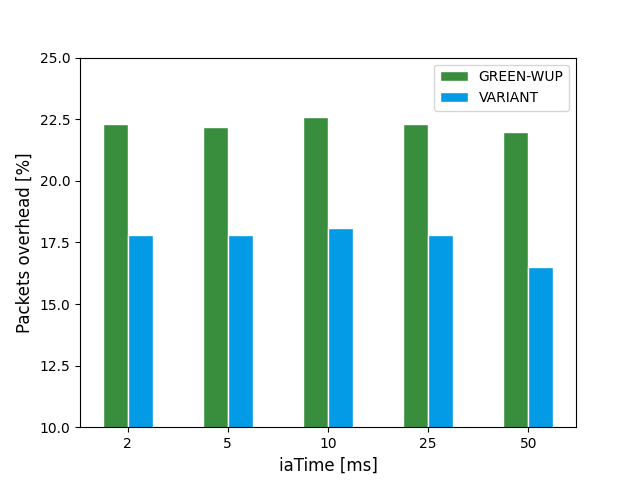
\includegraphics[width=1\linewidth]{overhead_plot.png}
        \caption*{(a)}
    \end{minipage}%
    \begin{minipage}{.5\textwidth}
        \centering
        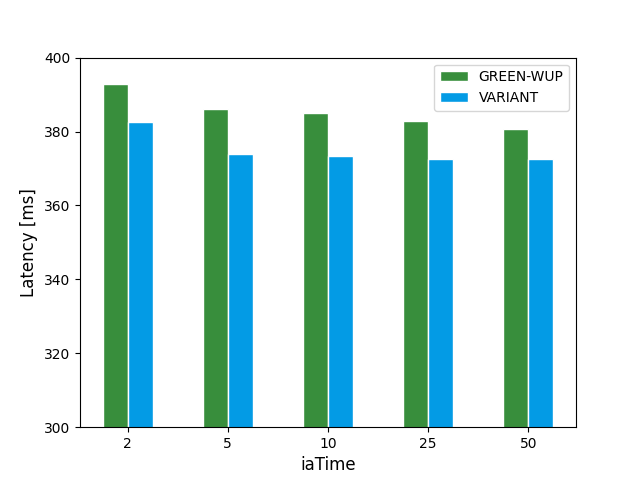
\includegraphics[width=1\linewidth]{latency_plot.png}
        \caption*{(b)}
    \end{minipage}
    \caption{Comparazione fra i due protocolli: (a) l'overhead di rete e (b) le latenze sperimentate.}
\end{figure}

Osservando la Figura 1.2 è evidente che l'overhead diminuisca nella variante proposta in quanto diminuisce il numero totale di pacchetti di controllo inviati
per garantire il corretto trasferimento dei pacchetti dati. Si può notare come questo scenda dal 22.3\% medio richiesto dall'implementazione originale
di GREEN-WUP al 17.5\% medio richiesto dalla variante. In particolare, il numero dei pacchetti CTS inviati è di circa il 27\% in meno rispetto
al precedente approccio e questa è una diretta conseguenza del fatto che in questo caso un minor numero di nodi viene coinvolto ad ogni step di
selezione del nodo intermedio. In altri termini, con la variante proposta si vogliono ridurre i nodi coinvolti allo stretto necessario per permettere
una corretta selezione del \emph{relay node} e contemporaneamente evitare sprechi energetici. Conseguentemente, la latenza media richiesta per far
recapitare un pacchetto dati al sink node è più bassa nella variante, in quanto minore il numero di pacchetti in circolazione e quindi nei buffer
dei nodi della rete.\\

\clearpage
\begin{figure}
    \centering
    \begin{minipage}{.5\textwidth}
        \centering
        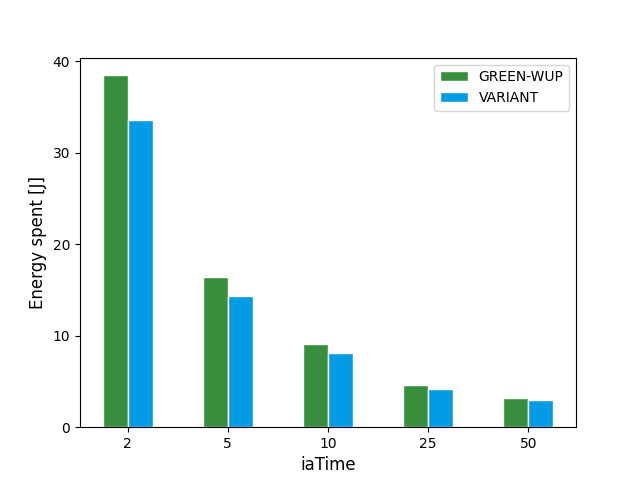
\includegraphics[width=1\linewidth]{energy_plot.png}
        \caption*{(a)}
    \end{minipage}%
    \begin{minipage}{.5\textwidth}
        \centering
        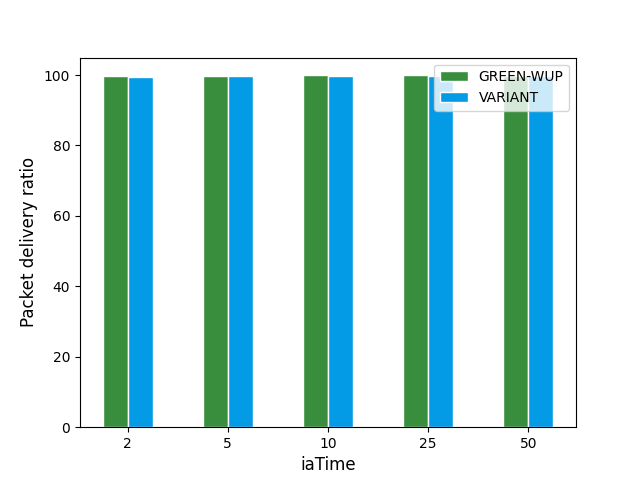
\includegraphics[width=1\linewidth]{pdr_plot.png}
        \caption*{(b)}
    \end{minipage}
    \caption{Comparazione fra i due protocolli: (a) l'energia spesa dalla rete e (b) il packet delivery ratio.}
\end{figure}

Analizzando la Figura 1.3 si può notare come l'energia richiesta dalla rete è inferiore nel caso della variante. Come diretta conseguenza di quanto 
sopra esposto, i consumi energetici sono ridotti in quanto i nodi della rete rispondono alle sequenze di wake up con sematic addressing in
numero minore rispetto alla versione originale. In particolare, la massima efficienza energetica è raggiunta in condizioni di maggiore stress
della rete in quanto maggiore la probabilità che un più alto numero di messaggi di wake up con semantic addressing svegli i nodi candidati. In altri
termini, la rete subisce un forte aumento dei pacchetti in circolazione, e quindi di messaggi di wake up, e in questo scenario gli effetti della
modifica che permette ai nodi di scegliere se attivare o meno la radio principale è ancor più evidente. L'efficienza energetica è favorita non solo
da questa modifica ma anche dalla stessa applicazione di jitter che vengono calcolati a partire dallo stato dei nodi
e che non sono puramente randomici come nel caso di GREEN-WUP.\\

Tutti i dati riportati fanno riferimento ad un numero di esecuzioni sufficientemente elevato da fornire un intervallo di confidenza del 95\% con una precisione
del 5\% e i risultati finali sono considerati come la media di tutte le esecuzioni.

\phantomsection % Give this command only if hyperref is loaded
\end{document}